\section{Deadlockerkennung allgemein}
\label{section:Deadlockerkennung allgemein}
Im Gegensatz zu Single-Threaded-Applikationen sind Multi-Threaded-Anwendungen
nicht deterministisch. Dies kann zu \textit{race conditions} führen. Eine
\textit{race condition} tritt zum Beispiel dann auf, wenn zwei Threads einen
Zähler jeweils um eins erhöhen wollen. Angenommen der Zähler hat zu Beginn den
Wert drei. Beide Threads wollen jetzt nahezu gleichzeitig den Zähler um eins
erhöhen. Dazu lesen beide Threads den aktuellen Wert des Zählers, in diesem Fall
drei, aus. Anschließend addieren beide eins hinzu und schreiben den neuen Wert,
in diesem Fall vier, in den Zähler. Erwartet wurde jedoch der Wert fünf, da
beide Threads den Zähler um jeweils eins erhöhen sollten. Um solche \textit{race
conditions} zu verhindert werden Synchronisierungsmechanismen benötigt.

Eine Möglichkeit um den Zugriff auf eine gemeinsame Ressource zu synchronisieren
sind Locks. Ein Lock ist ein exklusiver Zugriff auf ein Objekt, ein sogenanntes
Lockobjekt. Das bedeutet, dass während ein Thread einen Lock auf ein Objekt
besitzt, andere Threads, welche auf dasselbe Objekt zugreifen wollen, warten
müssen bis es freigegeben wurde.

Betrachtet man das Beispiel mit dem Zähler erneut, dieses Mal mit Locks als
Synchronisationsmittel, kann es zu folgender Ausführung kommen. Der Zähler hat
zu Beginn wieder den Wert drei. Die Threads \textit{T1} und \textit{T2} wollen
erneut den Zähler nahezu gleichzeitig erhöhen. Dieses Mal versuchen beide das
Lockobjekt \textit{L1} in Besitz zu nehmen. Der Thread \textit{T2} nimmt
\textit{L1} zuerst in Besitz, daraus folgt \textit{T1} muss warten. \textit{T2}
liest den aktuellen Wert des Zählers aus, erhöht diesen um eins und schreibt den
neuen Wert vier in den Zähler. Anschließend gibt \textit{T2} das Lockobjekt
\textit{L1} frei. Jetzt erhält der Thread \textit{T1} den Zugriff auf
\textit{L1} und liest ebenfalls den Zähler, jetzt vier, aus, erhöht diesen und
schreibt den neuen Wert fünf in den Zähler. Anschließend gibt \textit{T1} das
Lockobjekt \textit{L1} frei.

Die Verwendung von Locks kann in Verbindung mit der nicht deterministischen
Ausführung von Multi-Threaded-Anwendungen zu Problemen führen. Angenommen es
existieren zwei Threads \textit{T1} und \textit{T2} und zwei Lockobjekte
\textit{L1} und \textit{L2}. Angenommen \textit{T1} besitzt \textit{L1} und zu
gleichen Zeit erlangt \textit{T2} das Lockobjekt \textit{L2}. Wenn jetzt der
Thread \textit{T1} das Lockobjekt \textit{L2} anfordert und der Thread
\textit{T2} das Lockobjekt \textit{L1}, kommt es zu einem \textit{Deadlock}. Die
Ausführung des Programms terminiert nicht, da beide Threads auf den jeweils
anderen Thread warten und sich gegenseitig blockieren.

Solche potenziellen Deadlocks zu erkennen ist die Aufgabe von statischen und
dynamischen Methoden zur Deadlockerkennung. Die statische Deadlockerkennung
analysiert den Quellcode und wird hier nicht näher betrachtet. Die dynamische
Deadlockerkennung analysiert eine Anwendung zur Laufzeit und läuft in folgenden
drei Schritten ab:
\begin{enumerate}
  \item Erstellung einer Trace-Datei
  \item Erstellung eines Graphen basierend auf den Informationen aus der
  Trace-Datei
  \item Auffinden von potenziellen Deadlocks durch die Identifizierung von
  Zyklen innerhalb des Graphen
\end{enumerate}

Eine Trace-Datei enthält einen \textit{execution
trace}\label{text:ExecutionTrace} des ausführenden Programms. Ein
\textit{execution trace} ist eine Abfolge von Events. Ein Event
\textit{e\textsubscript{i}} wird durch eine der folgenden Methoden definiert:
starten eines Threads, Inbesitznahme eines Lockobjekts und Freigabe eines
Lockobjekts. Das Starten eines neues Threads ist definiert durch ein
Thread-Start-Event:
\begin{quote}
\texttt{s(ausführender Thread, Name des neuen Threads)}
\end{quote}
Zum Beispiel bedeutet \texttt{s(main,T1)}, dass der Thread \textit{main} den
Thread \textit{T1} gestartet hat. Die Inbesitznahme eines Lockobjekts ist
definiert durch ein Lock-Event:
\begin{quote}
\texttt{l(ausführender Thread, Name des Lockobjekts)}
\end{quote}
Zum Beispiel bedeutet \texttt{l(T1,L3)}, dass der Thread \textit{T1} das
Lockobjekt \textit{L3} in Besitz genommen hat. Die Freigabe eines Lockobjekts
ist definiert durch ein Unlock-Event:
\begin{quote}
\texttt{u(ausführender Thread, Name des Lockobjekts)}
\end{quote}
Zum Beispiel bedeutet \texttt{u(T1, L3)}, dass der Thread \textit{T1} das
Lockobjekt \textit{L3} freigegeben hat.

Die Abfolge aller während der Laufzeit des Programms aufgetretenen Events
definieren einen möglichen \textit{execution trace} des Programms. Programme
welche mit mehreren Threads arbeiten, liefern keine deterministische Abfolge.
Jede Ausführung eines solchen Programms kann zu unterschiedlichen
\textit{execution traces} führen. 

Im zweiten Schritt wird aus dem vorher erzeugten \textit{execution trace} ein
Lockgraph erstellt. Ein Lockgraph ist definiert durch:
\begin{quote}
\textbf{LG} = (L,R)
\end{quote}
\textit{L} ist die Menge aller Lockobjekte im \textit{execution trace} und
\textit{R} die Menge aller Lockpaare. Ein Lockpaar ist definiert durch das Tupel
\textit{(L1, L2} für das gilt: Es existiert ein Thread, welcher das Lockobjekt
\textit{L1} besitzt, während er den Lock \textit{L2} anfordert.

\section{PEARL}
\label{section:PEARL}
Die Programmiersprache PEARL wurde in den 1970er Jahren vom Institut für
Regelungstechnik der Universität Hannover entwickelt \autocite{PEARLHistory}.
PEARL ist eine Abkürzung und steht für "Process and Experiment Automation
Realtime Language". Die Programmiersprache erlaubt eine komfortable, sichere und
weitgehend rechnerunabhängige Programmierung von Multitasking- und
Echtzeit-Aufgaben. Das Deutsche Institut für Normung standardisierte PEARL
mehrmals, unteranderem 1998 in der DIN 66253-2 als PEARL90
\autocite{DIN-66253-2:1998-04} und zuletzt 2018 als SafePEARL
\autocite{DIN-66253:2018-03}. Nachfolgend werden PEARL und PEARL90 synonym
verwendet. 

In PEARL bezeichnet ein \textit{TASK} eine Aufgabe und wird entweder direkt beim
Start des Programms oder durch Signale von anderen Aufgaben gestartet.
\textit{TASKs} werden parallel und gemäß ihrer Priorität ausgeführt. Um mehrere
\textit{TASKs} zu synchronisieren gibt es zwei Möglichkeiten: \textit{SEMA} und
\textit{BOLT} Variablen. 

Eine \textit{SEMA} Variable ist ein Semaphore und dient als
Synchronisationsmittel. Sie kann als Wert nicht negative ganze Zahlen besitzen,
wobei null den Zustand "gesperrt" und positive Zahlen den Zustand "frei"
bedeuten \autocite[9--17]{PEARL}. Eine \textit{SEMA} Variable hat zu Beginn den
Wert null und den Zustand "gesperrt". Mit dem Befehl \textit{RELEASE} wird eine
\textit{SEMA} Variable um den Wert eins erhöht und erhält den Zustand "frei".
Mit dem \textit{REQUEST} Befehl wird der Wert einer \textit{SEMA} Variablen um
eins verringert. Ist der Wert einer \textit{SEMA} Variablen null wird der
ausführende \textit{TASK} angehalten und in eine Warteschlange eingereiht.
Sobald die Variable über den Befehl \textit{RELEASE} wieder freigeben wird, wird
der nächste \textit{TASK} in der Warteschlange gemäß seiner Priorität
fortgeführt. Das Zustandsdiagramm zur \textit{SEMA} Variable ist in
\cref{fig:SEMA_StateDiagram} dargestellt.

\begin{figure}[ht]
  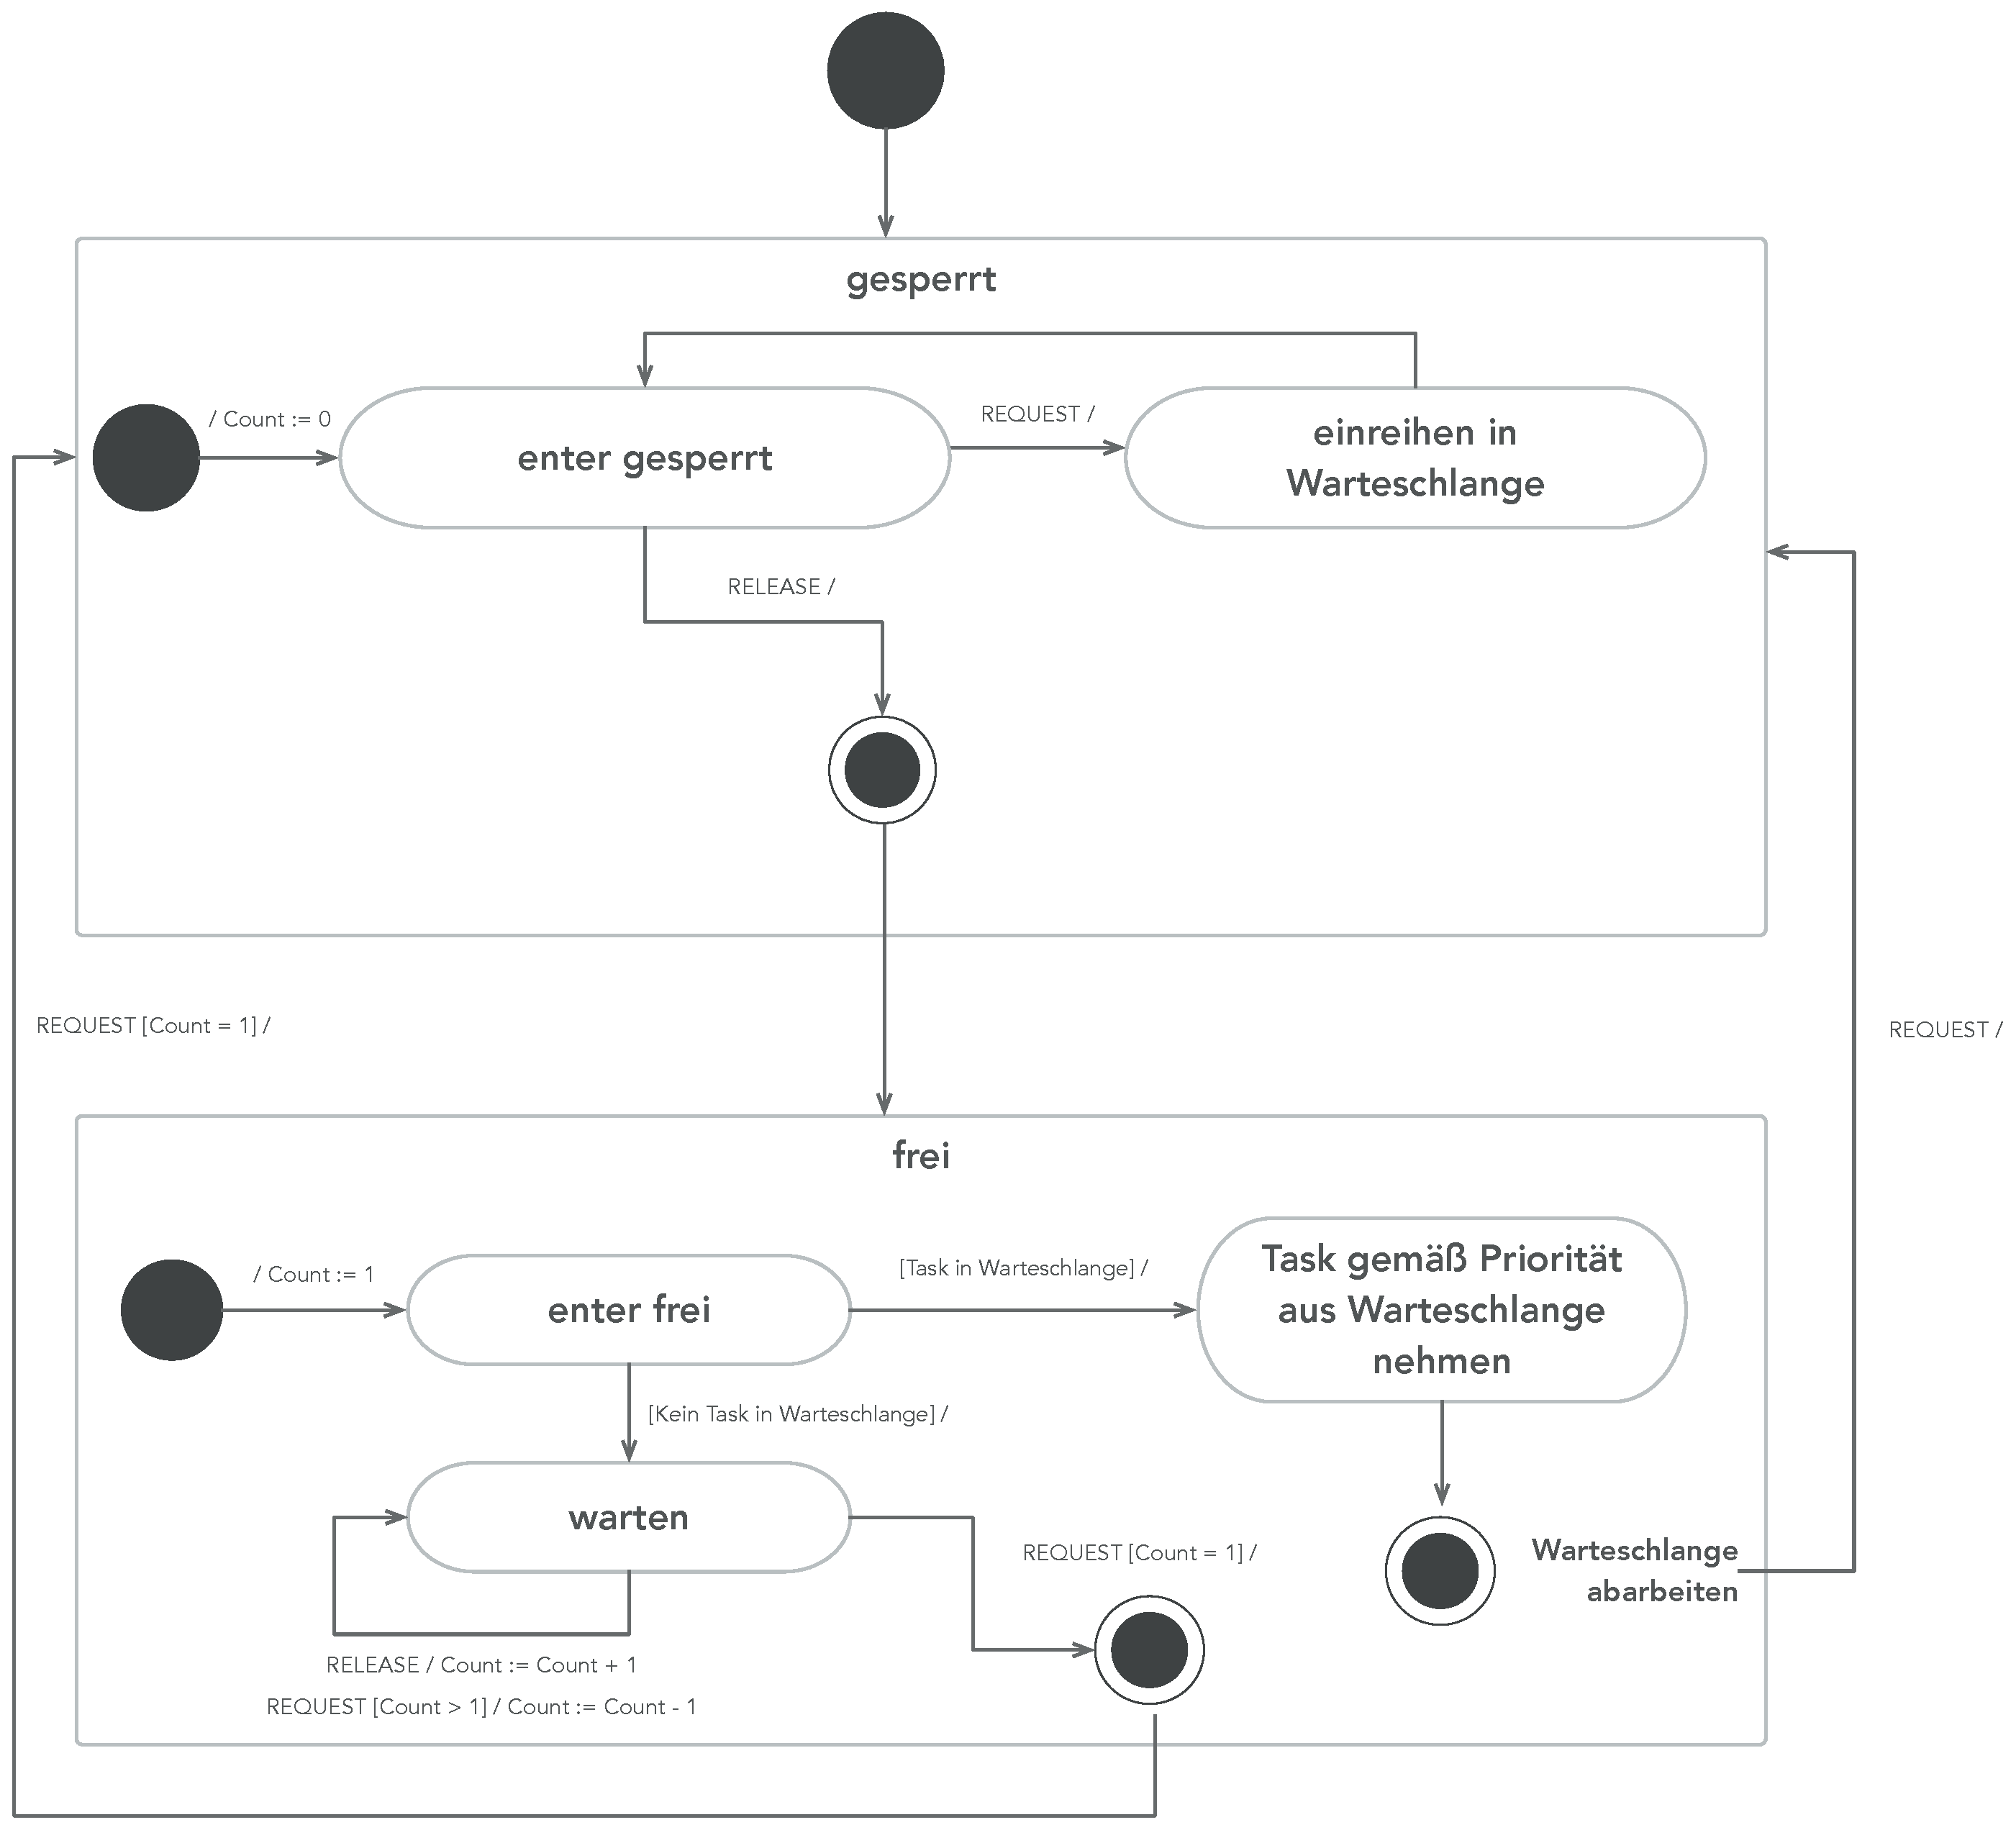
\includegraphics[width=\linewidth]{SEMA_State_Diagram.eps}
  \caption{Zustandsdiagramm einer SEMA Variablen}
  \label{fig:SEMA_StateDiagram}
\end{figure}

\textit{BOLT} Variablen haben im Gegensatz zu \textit{SEMA} Variablen drei
Zustände "gesperrt", "Sperre möglich" und "Sperre nicht möglich"
\autocite[9--17]{PEARL}. Sie bieten die Möglichkeit exklusive und nicht
exklusive Sperren zu ermöglichen. Zum Beispiel können so simultane Lesezugriffe
und exklusive Schreibzugriffe realisiert werden. Zu Beginn hat eine
\textit{BOLT} Variable den Zustand "Sperre möglich". Mit dem Befehl
\textit{RESERVE} wird ein exklusiver Zugriff auf eine \textit{BOLT} Variable
angefordert. Wenn die Variable im Zustand "Sperre möglich" ist, erhält diese den
Zustand "gesperrt". Ansonsten wird ähnlich zu der \textit{REQUEST} Anweisung für
\textit{SEMA} Variablen der ausführende \textit{TASK} angehalten und in eine
Warteschlange eingereiht. Mit dem Befehl \textit{FREE} erhält eine \textit{BOLT}
Variable den Zustand "Sperre möglich" und alle \textit{TASKs} in der
Warteschlange, welche aufgrund einer \textit{RESERVE} Anweisung warten, werden
gemäß ihrer Priorität fortgeführt. Wenn keine \textit{TASKs} in der
Warteschlange vorhanden sind, welche auf eine \textit{RESERVE} Anweisung warten,
werden die \textit{TASKs} in der Warteschlange gemäß ihrer Priorität
fortgeführt, welche aufgrund einer \textit{ENTER} Anweisung warten. Mit der
\textit{ENTER} Anweisung wird ein nicht exklusiver Zugriff angefordert. Wenn die
\textit{BOLT} Variable im Zustand "gesperrt" ist oder ein \textit{TASK} in der
Warteschlange existiert, welcher einen exklusiven Zugriff mittels einer
\textit{RESERVE} Anweisung angefordert hat, wird der ausführende \textit{TASK}
angehalten und in eine Warteschlange eingereiht. Ansonsten erhält ie Variable
den Zustand "Sperre nicht möglich", um den exklusiven Zugriff zu verbieten.
Zusätzlich wird die Anzahl der benutzenden \textit{TASKs} um eins erhöht. Die
\textit{LEAVE} Anweisung verringert die Anzahl der benutzenden \textit{TASKs} um
eins, wenn die Anzahl eins entspricht, funktioniert die \textit{LEAVE} Anweisung
wie die \textit{FREE} Anweisung. Das Zustandsdiagramm zur \textit{BOLT} Variable
ist in \cref{fig:BOLT_StateDiagram} dargestellt.

\begin{figure}[ht]
  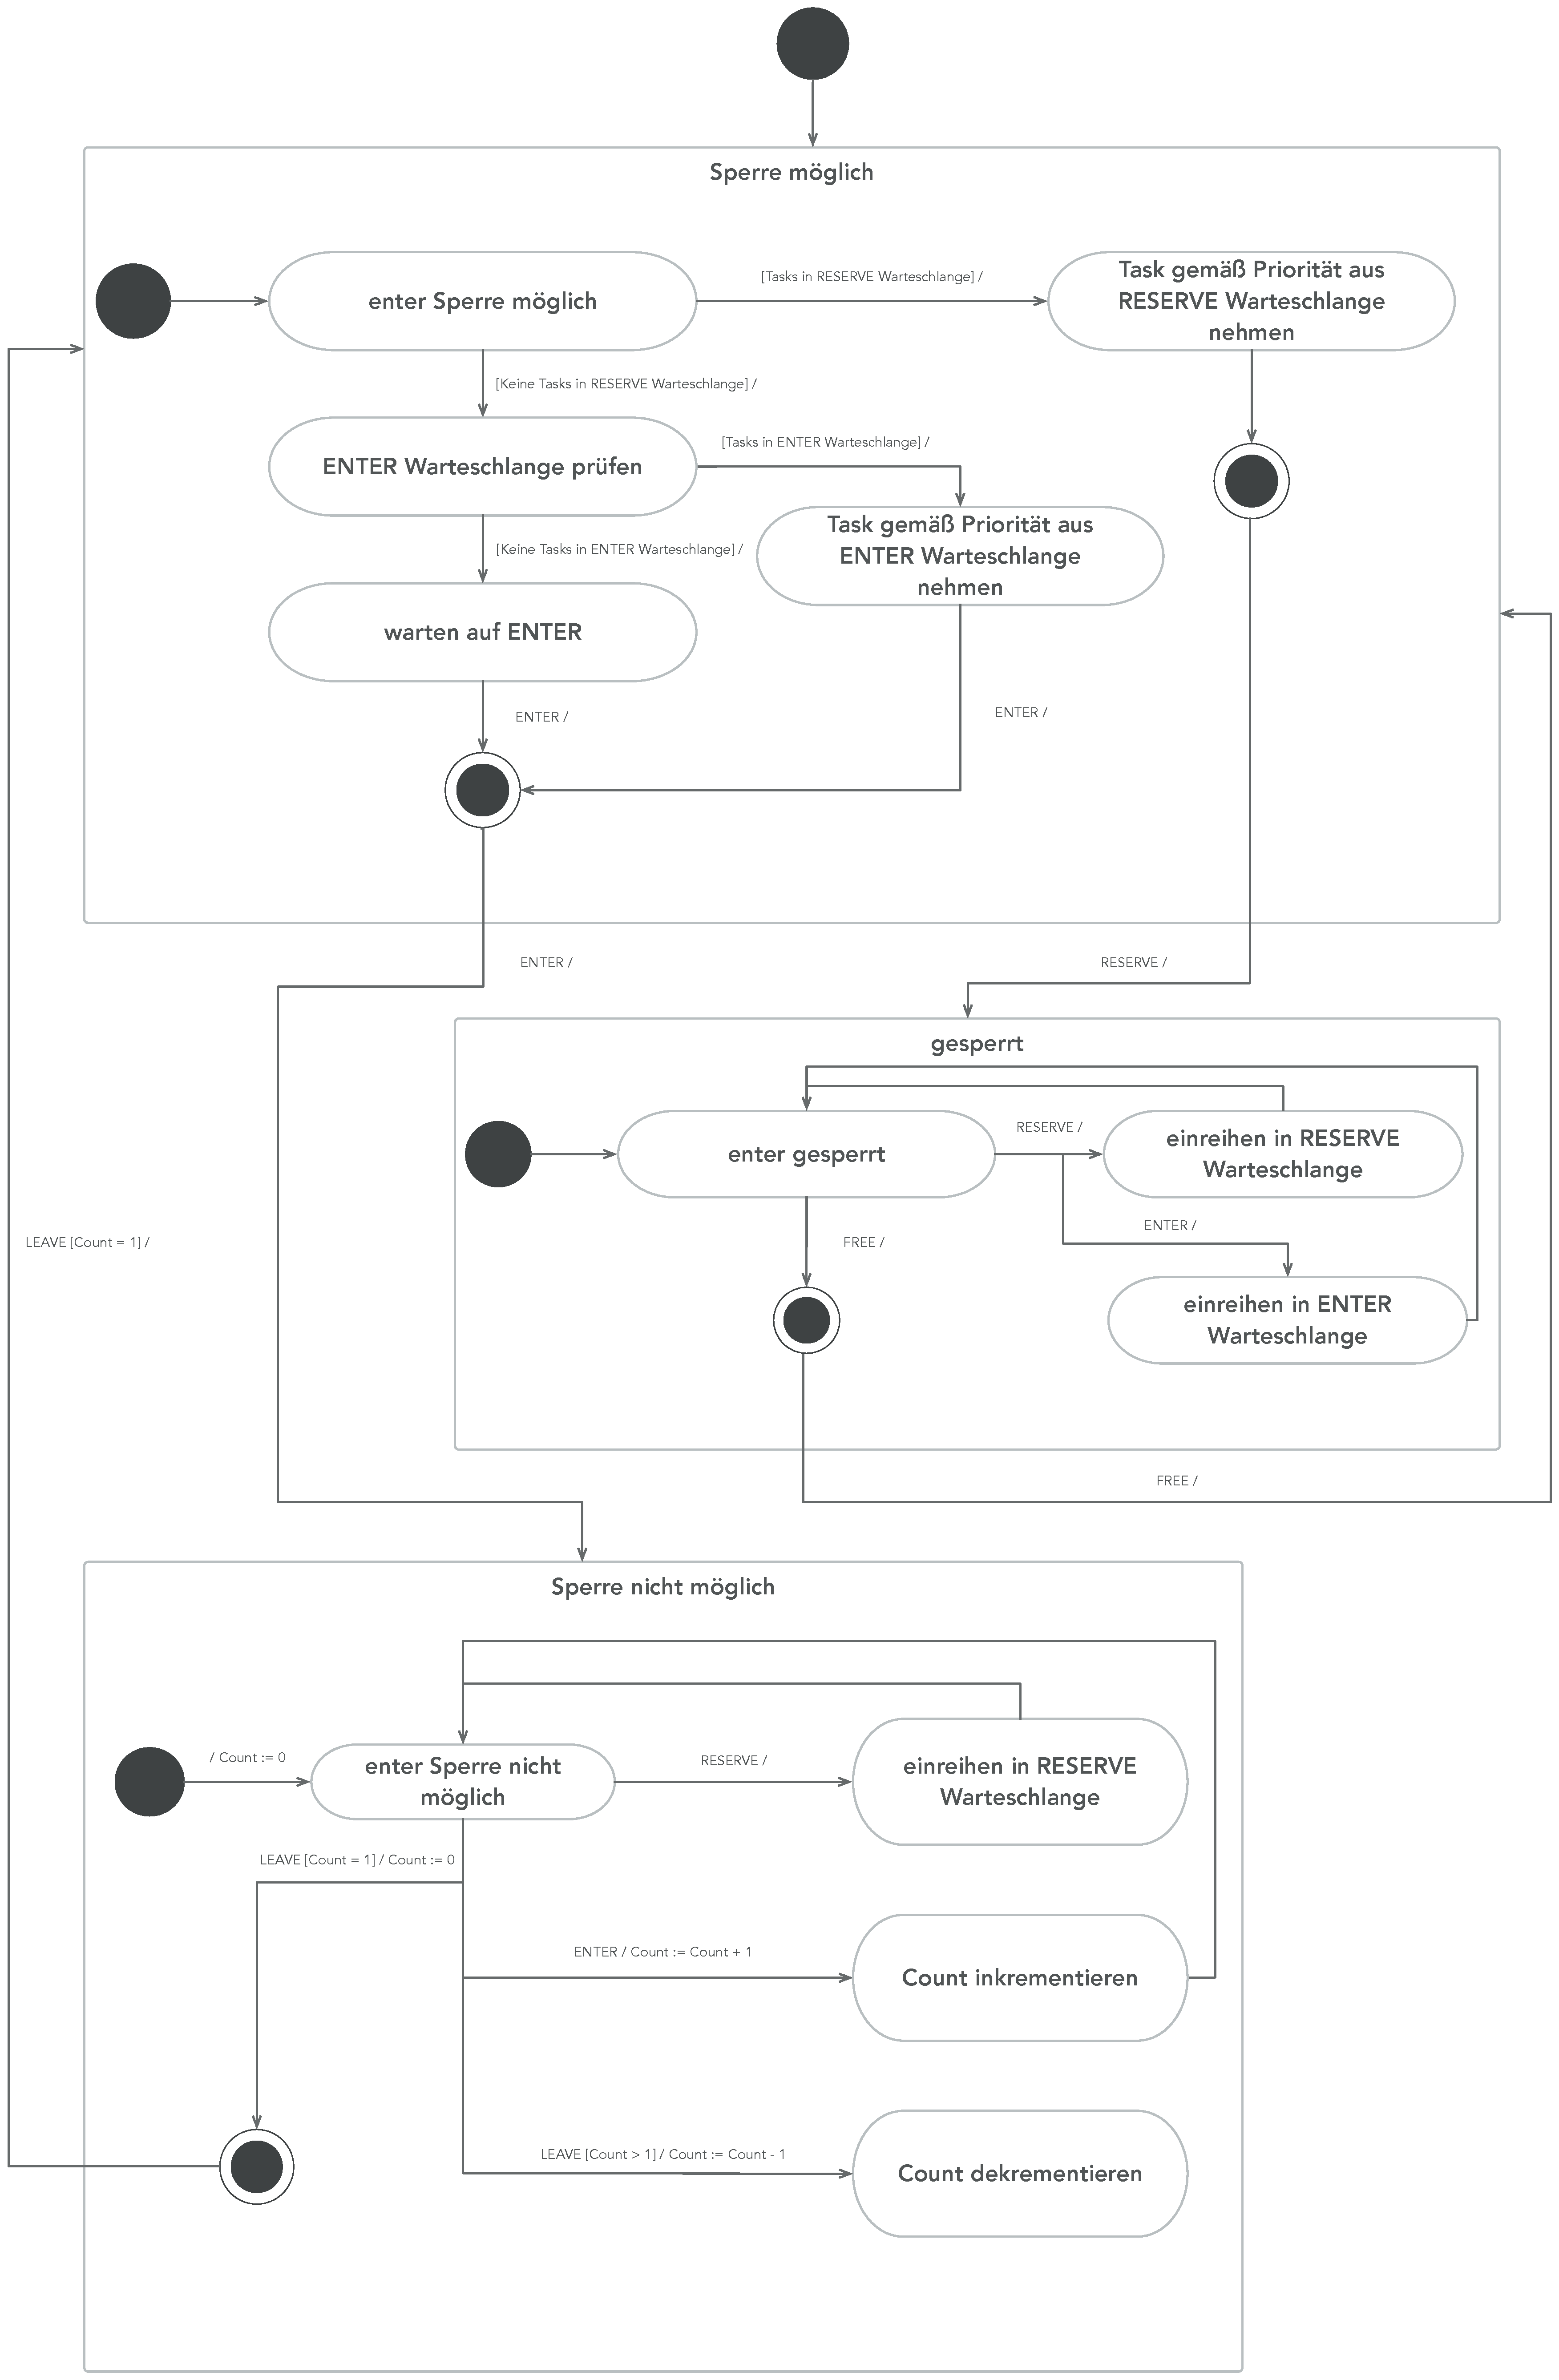
\includegraphics[width=\linewidth]{BOLT_State_Diagram.eps}
  \caption{Zustandsdiagramm einer BOLT Variablen}
  \label{fig:BOLT_StateDiagram}
\end{figure}

\section{OpenPEARL}
\label{section:OpenPEARL}
Um PEARL Programme auf einem System auszuführen wird ein Compiler benötigt. Das
OpenSource Projekt OpenPEARL besteht aus einem Compiler und einer
Laufzeitumgebung für PEARL \autocite{OpenPEARL}. Unterstützt wird der PEARL90
Standard bis auf einige wenige Unterschiede
\autocite{OpenPEARL_Differences_To_PEARL90}.

OpenPEARL besteht aus drei wesentlichen Komponenten:
\begin{enumerate}
  \item Compiler
  \item Laufzeitumgebung
  \item Inter Module Checker
\end{enumerate}
Der Compiler ist in Java geschrieben und übersetzt PEARL Code in C++ Code. Die
Laufzeitumgebung stellt dem Compiler eine API zur Verfügung. Dem Compiler werden
durch die API sichere Implementierungen der PEARL Datentypen zur Verfügung
gestellt. Zusätzlich enthält die Laufzeitumgebung plattformspezifische Anteile
für zum Beispiel die Implementierung für das Scheduling der Tasks. PEARL
Anwendungen können aus mehreren Modulen bestehen, welche unabhängig voneinander
kompiliert werden. Um Inkonsistenzen bei der Erstellung der Anwendung zu
verhindern, prüft der Inter Module Checker die Export- und Importschnittstellen
aller Module und prüft deren Kompatibilität.

In \cref{lst:ExampleDeadlock} ist ein Beispielprogramm in der Programmiersprache
PEARL dargestellt. Das Programm startet zwei parallele Aufgaben welche beide
eine Zeichenfolge auf der Standardausgabe ausgeben. Der Zugriff auf die
Standardausgabe muss dabei synchronisiert erfolgen.

\begin{listing}[ht]
  \inputminted[frame=lines,linenos]{vim}{./Examples/Example_Deadlock.prl}
  \caption{Beispiel einer OpenPEARL Anwendung mit einem potenziellen Deadlock}
  \label{lst:ExampleDeadlock}   
\end{listing} 

In den Zeilen 1 bis 11 werden Variablen definiert, wie zum Beispiel die Ausgabe
über die Standardausgabe und die zwei \textit{SEMA} Variablen \textit{L1} und
\textit{L2} in den Zeilen 9 und 10. In den Zeilen 12 bis 17 ist ein
\textit{TASK} definiert. Durch die Kennzeichnung \textit{MAIN} wird der
\textit{TASK} direkt beim Start des Programms ausgeführt. Die Befehle
\textit{RELEASE} in den Zeilen 13 und 14 erhöhen den Wert der jeweiligen
\textit{SEMA} Variable um eins, wodurch der Zustand von "gesperrt" auf "frei"
gesetzt wird. Anschließend werden in den Zeilen 15 und 16 die \textit{TASKS}
\textit{T2} und \textit{T3} gestartet.

Die \textit{TASKS} \textit{T2} und \textit{T3} geben in den Zeilen 22 bis 24 und
in den Zeilen 32 bis 34 die Zeichenfolge "Hello World T2" bzw. "Hello World T3"
auf der Standardausgabe aus. Die Synchronisierung des Zugriffs auf die
Standardausgabe erfolgt mittels den \textit{SEMA} Variablen \textit{L1} und
\textit{L2}. Beide \textit{TASKS} versuchen beide \textit{SEMA} Variablen in
Besitz zu nehmen. \textit{T2} versucht in den Zeilen 20 und 21 zuerst
\textit{L1} und dann \textit{L2} in Besitz zu nehmen. \textit{T3} versucht in
den Zeilen 30 und 31 zuerst \textit{L2} und dann \textit{L1} in Besitz zu
nehmen. Da beide \textit{TASKS} parallel laufen, kann es passieren, dass
\textit{T2} \textit{L1} in Zeile 20 in Besitz nimmt und gleichzeitig \textit{T3}
in Zeile 30 \textit{L2} in Besitz nimmt. Beide \textit{SEMA} Variablen haben
jetzt den Wert null und den Zustand "gesperrt". Der \textit{TASK} \textit{T2}
wartet jetzt darauf, dass \textit{L2} freigegeben wird und \textit{T3} wartet
darauf, dass \textit{L1} freigegeben wird. Beide \textit{TASKS} warten auf den
jeweils anderen. Diese Situation wird als Deadlock bezeichnet.

\section{MagicLock}
\label{section:MagicLock}
Der nachfolgende Abschnitt basiert auf den Ausführungen in \autocite{MagicLock}.

MagicLock ist ein Algorithmus zur dynamischen Deadlockerkennung. Während der
Entwicklung wurde der Fokus auf die Skalierung und Effizienz des Algorithmus
gesetzt. Ziel war es mit großen Multithreaded Anwendungen skalieren und diese
effizient analysieren zu können.

MagicLock analysiert einen \textit{execution trace}\footnote{siehe
\cref{text:ExecutionTrace}} einer Programmausführung ohne Deadlocks. Ein
möglicher \textit{execution trace} von dem Beispielprogramm aus
\cref{lst:ExampleDeadlock} ist:
\begin{quote}
  \textbf{$\sigma$} = s(main,T1), u(T1,L1), u(T1,L2), s(T1,T2), s(T1,T3),
  l(T2,L1), l(T2,L2), u(T2,L2), u(T2,L1), l(T3,L2), l(T3,L1), u(T3,L1), u(T3,L2)
\end{quote}
Der \textit{execution trace} in MagicLock wird durch eine
Lock-Dependency-Relation definiert. Eine Lock-Dependency-Relation D besteht aus
einer Sequenz von Lock-Dependencies. Eine Lock-Dependency ist ein Triple
\textit{r = (t,m,L)} in dem \textit{t} ein Thread ist, \textit{m} ein
Lock-Objekt und \textit{L} eine Menge von Lock-Objekten. Das Triple sagt aus,
dass der Thread \textit{t} das Lock-Objekt \textit{m} in Besitz nimmt, während
er jedes Lock-Objekt in \textit{L} besitzt.

Bei einem Thread-Start-Event wird ein neuer Thread-Identifier und eine leere
Menge an Locks für den neu erzeugten Thread erstellt. Zum Beispiel wird bei den
Event \textit{s(main,T1)} ein neuer Thread-Identifier für T1 erzeugt und eine
leere Menge L\textsubscript{T1}. Bei einem Lock-Event \textit{l(T2,L1)} wird
zuerst die Lock-Dependency \textit{(T2,L1,L\textsubscript{T2})} an den
\textit{execution trace} angehängt und anschließend L1 in die Menge der Locks
L\textsubscript{T2} eingefügt. Bei einem Unlock-Event \textit{u(T2,L2)} wird das
Lock-Objekt L2 aus der Menge L\textsubscript{T2} entfernt. Daraus folgt die
Lock-Dependency-Relation:
\begin{quote}
  \textbf{$D_\sigma$} = (T2,L1,\{\}), (T2,L2,\{L1\}), (T3,L2,\{\}),
  (T3,L1,\{L2\})
\end{quote}
Anschließend wird ein reduzierter \textit{execution trace} erzeugt. Dazu
verwendet MagicLock einen Algorithmus zur Reduzierung von Lock-Objekten im
\textit{execution trace}. Der Algorithmus entfernt alle Lock-Objekte aus der
Menge aller Lock-Objekte \textit{Locks} aus \textit{$D_\sigma$} die entweder
keine eingehenden \textit{indegree(m) = 0} oder keine ausgehenden
\textit{outdegree(m) = 0} Kanten im Lockgraph besitzen. Die Annahme ist, dass
ein Lock-Objekt nur Teil eines Zyklus sein kann, wenn dieses mindestens eine
eingehende und mindestens eine ausgehende Kante besitzt. Zusätzlich werden alle
Lock-Objekte entfernt, welche nur von einem einzigen Thread in Besitz genommen
bzw. freigegeben wurden. Wenn nur ein Thread ein Lock-Objekt benutzt, kann
dieses Lock-Objekt nicht Teil eines Deadlocks sein. Mit den reduzierten
Lock-Objekten wird im nächsten Schritt die Zyklensuche vorbereitet.

Die noch vorhandenen Lock-Dependencies werden in Partitionen basierend auf ihrer
Thread ID unterteilt und anschließend sortiert. Für jeden Thread wird eine
Partition erstellt mit allen Lock-Dependencies mit \textit{($t_i$,m,L)} wobei
\textit{$t_i$} der jeweilige Thread der Partition ist. Zusätzlich werden gleiche
Lock-Dependencies in Gruppen eingeteilt. Für gleiche Lock-Dependencies muss dann
immer nur ein Element aus der Gruppe geprüft werden. Wenn ein Zyklus gefunden
wurde, wurde gleichzeitig ein Zyklus für alle Lock-Dependencies in der Gruppe
gefunden. Wenn kein Zyklus gefunden wurde, wird dies gleichzeitig für alle
anderen Elemente in der Gruppe angenommen. Zwei Lock-Dependencies sind gleich
wenn gilt:
\begin{quote}
  Gegeben sind zwei Lock-Dependencies \textit{$T_1 = (t_1, m_1, L_1)$} und
  \textit{$T_2 = (t_2, m_2, L_2)$}: $T_1 = T_2 \Leftrightarrow t_1 = t_2 \land
  m_1 = m_2 \land L_1 = L_2 $
\end{quote}
Anschließend werden die Partitionen gegeneinander auf Lock-Dependency-Chains
geprüft. Eine Lock-Dependency-Chain ist eine Sequenz von Lock-Dependencies für
die gilt:
\begin{quote}
  \textbf{$d_{chain}$} = $(T_1, T_2, \dots , T_k)$ mit $T_i = (t_i, m_i, L_i)$,
  wenn $m_1 \in L_2 \dots m_{k-1} \in L_k, t_i \neq t_j$ und $L_i \cap L_j =
  \emptyset$ für $1 \leq i, j \leq k (i \neq j)$
\end{quote}
Zum Beispiel ist die Lock-Dependency Sequenz \textit{$d = (t_1, l_2, \{l_1\}),
(t_2, l_1, \{l_2\})$} eine Lock-Dependency-Chain. Jede Lock-Dependency-Chain
repräsentiert einen potenziellen Deadlock.